\chapter{Results}
This chapter shows the results for the following experiments.

\begin{enumerate}
Reconstruction quality is mean of PSNR of images inside and outside of the
training sets.
 \item Convergence of reconstruction quality for different training parameters.
 \item Inspection of the structures of dictionary atoms from different
groups of images and block size and win size.
 \item Comparision of reconstruction quality of different sizes of dictionaries
in single and in cluster. 
 \item Compression quality of natural images and sketches dict. vs.
JPEG/JPEG2000 of images.
\end{enumerate}

We discuss the results in the next chapter.

%\section{Quality}
%\subsection*{trained vs. analytical base}
%\subsection*{Compression ratio}
%\subsection*{Dictionary size}
%Setup:
%  initialize: random pixels, radom samples 
%  dict size: 256, 1000, 4000, 8000
%  coeffs: 5, 10, 20

\section{Dictionary size}
\begin{table}[h]
\caption{dictionary size}
\centering
\begin{tabular}{l  c  c  c  c  c}
\toprule
Image & 1 & 2 & 3 & 4 & 5 \\
\hline
300 & 30 & 30 & 30 & 30 & 30 \\
600 & 30 & 30 & 30 & 30 & 30 \\
900 & 30 & 30 & 30 & 30 & 30 \\
1800 & 30 & 30 & 30 & 30 & 30 \\
3000 & 30 & 30 & 30 & 30 & 30 \\
\bottomrule
\end{tabular}
\end{table}

\Todo{small image sample comparision}
\begin{figure}[h]
\centering
\subfloat[300]{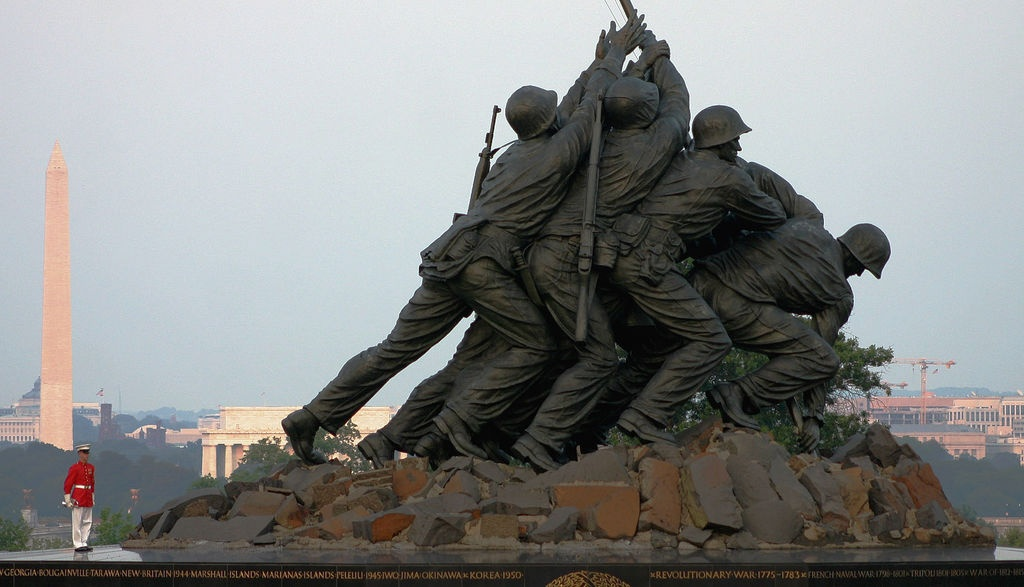
\includegraphics[width = 0.3\textwidth]{images/28979823.jpg}}
\hspace{5mm}
\subfloat[900]{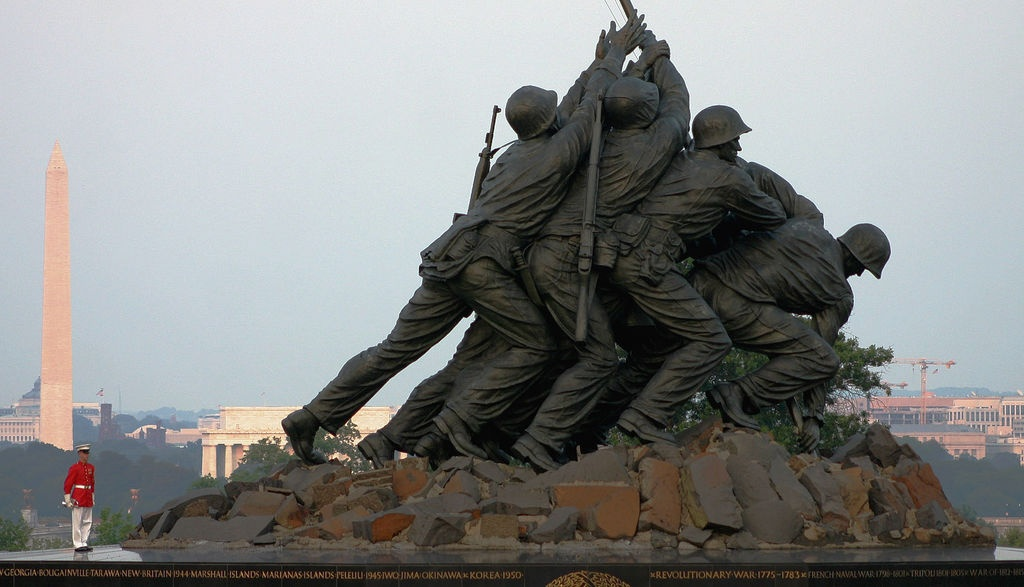
\includegraphics[width = 0.3\textwidth]{images/28979823.jpg}}
\hspace{5mm}
\subfloat[3000]{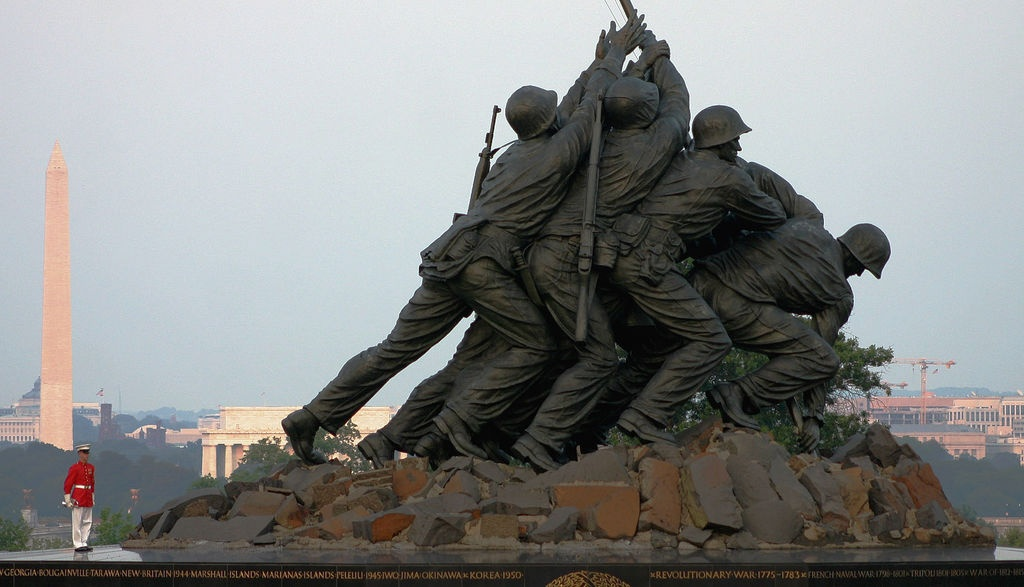
\includegraphics[width = 0.3\textwidth]{images/28979823.jpg}}
\caption{dict size differences on sub region of image}
\label{fig:dict size}
\end{figure}

\section{Single vs. Cluster}
\begin{table}[H]
\caption{single vs. cluster}
\centering
\begin{tabular}{l c c c c c}
\hline\hline
Image & 300 & 600 & 900 & 1800 & 3000 \\
\hline
image 1 & 30 & 30 & 30 & 30 & 30 \\
image 2 & 30 & 30 & 30 & 30 & 30 \\
image 3 & 30 & 30 & 30 & 30 & 30 \\
\hline
\end{tabular}
\end{table}

\begin{figure}[H]
\centering
\subfloat[low pass]{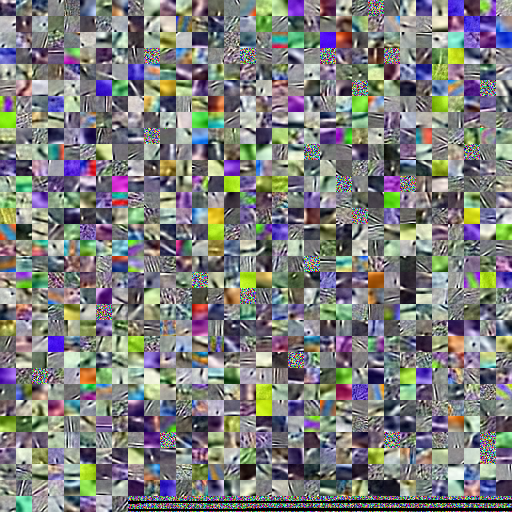
\includegraphics[width =
0.4\textwidth]{images/16_1000_1000_10_lasso.png}}
\hspace{5mm}
\subfloat[high pass]{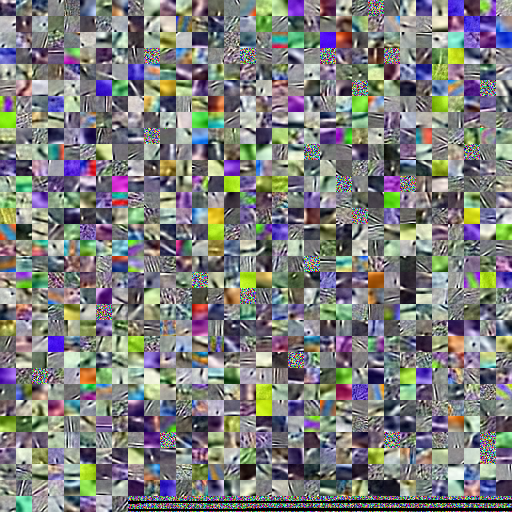
\includegraphics[width =
0.4\textwidth]{images/16_1000_1000_10_lasso.png}}
\caption{low pass}
\label{fig:16_1000_lasso}
\end{figure}
\begin{figure}
\centering
\subfloat[low pass]{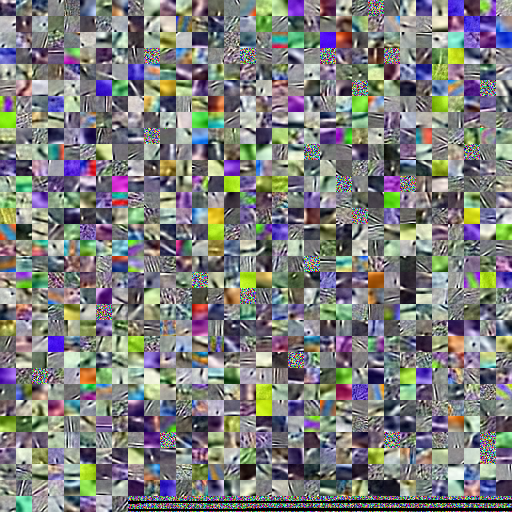
\includegraphics[width =
0.4\textwidth]{images/16_1000_1000_10_lasso.png}}
\hspace{5mm}
\subfloat[high pass]{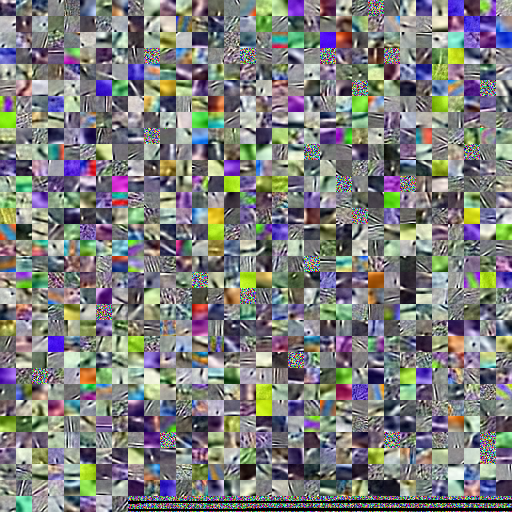
\includegraphics[width =
0.4\textwidth]{images/16_1000_1000_10_lasso.png}}
\caption{low pass}
\label{fig:16_1000_lasso}
\end{figure}
\begin{figure}
\centering
\subfloat[low pass]{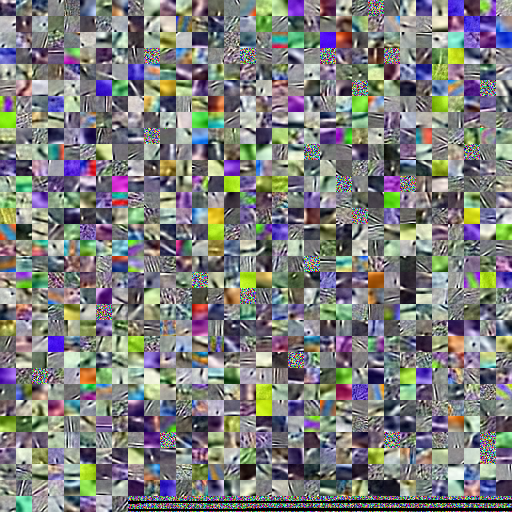
\includegraphics[width =
0.4\textwidth]{images/16_1000_1000_10_lasso.png}}
\hspace{5mm}
\subfloat[high pass]{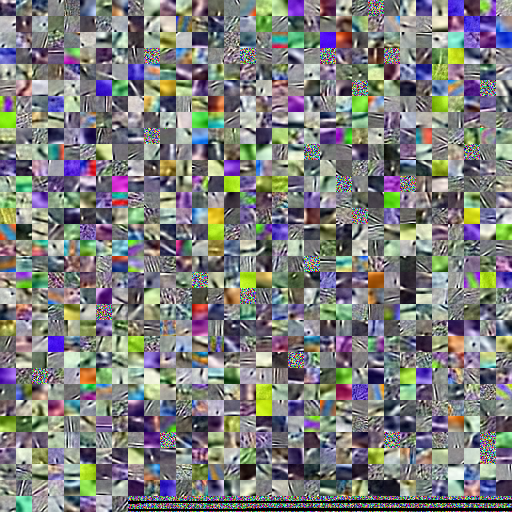
\includegraphics[width =
0.4\textwidth]{images/16_1000_1000_10_lasso.png}}
\caption{low pass}
\label{fig:16_1000_lasso}
\end{figure}

\section{Dictionary elements}
\begin{figure}[H]
\centering
\subfloat{
\includegraphics[width = 0.3\textwidth]{images/gradient.png}}
\hspace{5mm}
\subfloat{
\includegraphics[width = 0.3\textwidth]{images/checkerboard.png}}
\hspace{5mm}
\subfloat{
\includegraphics[width = 0.3\textwidth]{images/spot.png}}
\hspace{5mm}
\subfloat{
\includegraphics[width = 0.3\textwidth]{images/edges.png}}
\hspace{5mm}
\subfloat{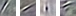
\includegraphics[width = 0.3\textwidth]{images/wavelet.png}}
\caption{image from database}
\label{fig:USC-SIPI}
\end{figure}

\section{Compression}

\subsection{Natural image database}


\begin{figure}[H]
\centering
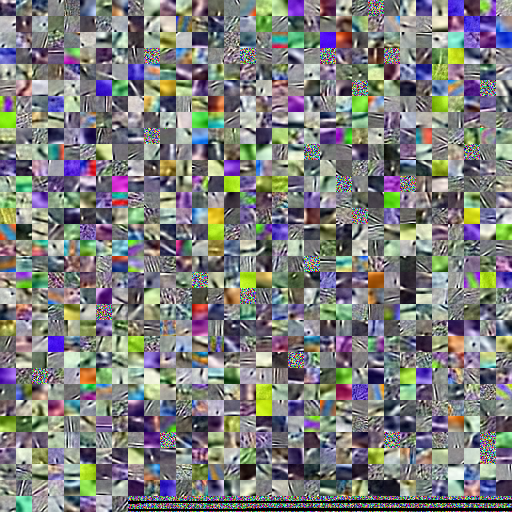
\includegraphics[width = 0.44\textwidth]{images/16_1000_1000_10_lasso.png}
\caption{16x16 LARS-lasso with 1000 elements}
\label{fig:16_1000_lasso}
\end{figure}

\begin{figure}[H]
\centering
\subfloat[low pass]{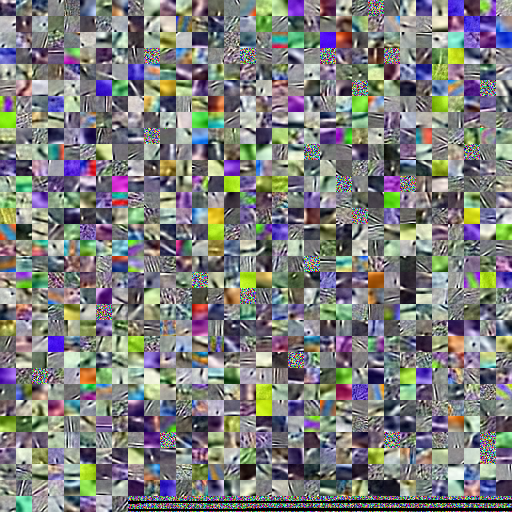
\includegraphics[width =
0.4\textwidth]{images/16_1000_1000_10_lasso.png}}
\hspace{5mm}
\subfloat[high pass]{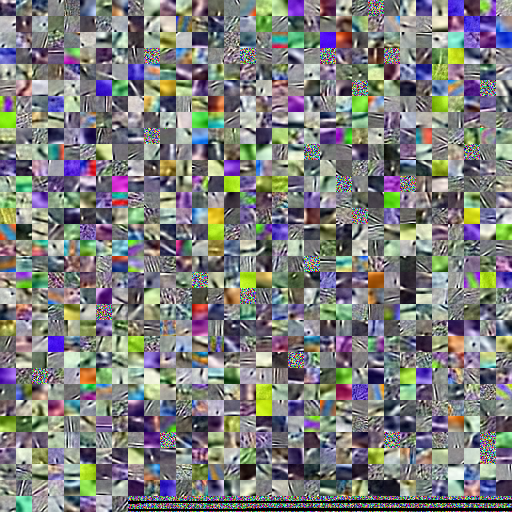
\includegraphics[width =
0.4\textwidth]{images/16_1000_1000_10_lasso.png}}
\caption{low pass}
\label{fig:16_1000_lasso}
\end{figure}
\begin{figure}[H]
\centering
\subfloat[low pass]{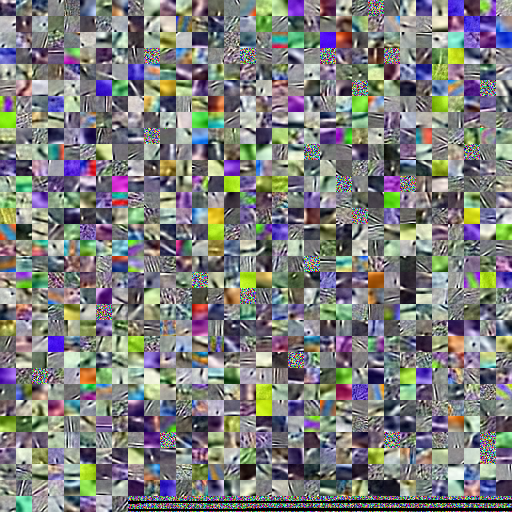
\includegraphics[width =
0.4\textwidth]{images/16_1000_1000_10_lasso.png}}
\hspace{5mm}
\subfloat[high pass]{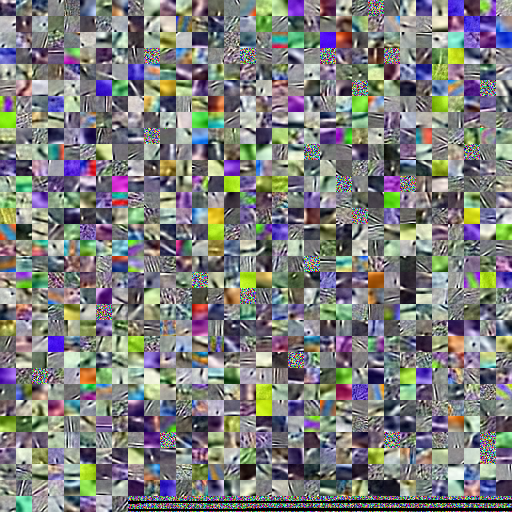
\includegraphics[width =
0.4\textwidth]{images/16_1000_1000_10_lasso.png}}
\caption{low pass}
\label{fig:16_1000_lasso}
\end{figure}
\begin{figure}[H]
\centering
\subfloat[low pass]{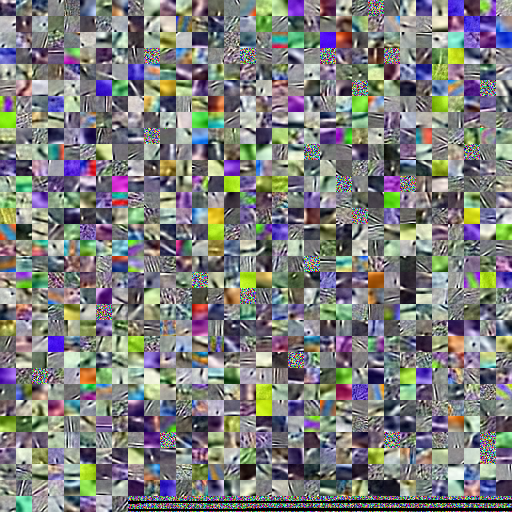
\includegraphics[width =
0.4\textwidth]{images/16_1000_1000_10_lasso.png}}
\hspace{5mm}
\subfloat[high pass]{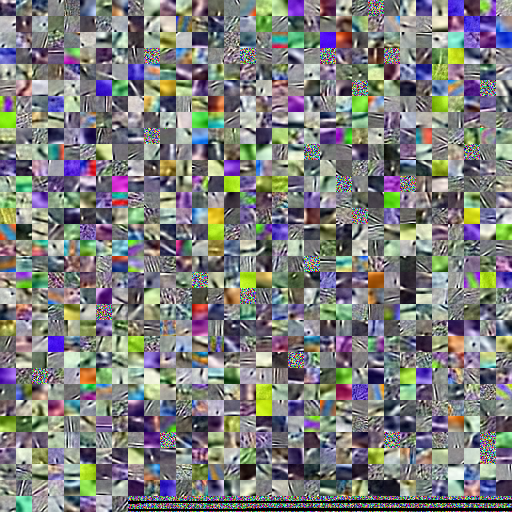
\includegraphics[width =
0.4\textwidth]{images/16_1000_1000_10_lasso.png}}
\caption{low pass}
\label{fig:16_1000_lasso}
\end{figure}



%\subsection{Specific image groups}










